\section{Motivation}

During the last couple of years a lot of software is moving from desktop to the web.

Many tasks can be now performed using only the web browser. A project called Chromebook \citep{chromebook} introduced a laptop which contains only a web browser and all the work is done using web applications.

That makes development and use of software better in many ways: Web applications are faster to implement, it is easier to customize their interfaces (using CSS), it is not necessary to download new versions of software as they are released and the data are stored and processed by the server.

When the data are stored on the server, they are stored more safely than on user's hard drive. Thanks to the client-server architecture, features for sharing and communication between users become trivial to implement.

\begin{figure}[ht!]
\centering
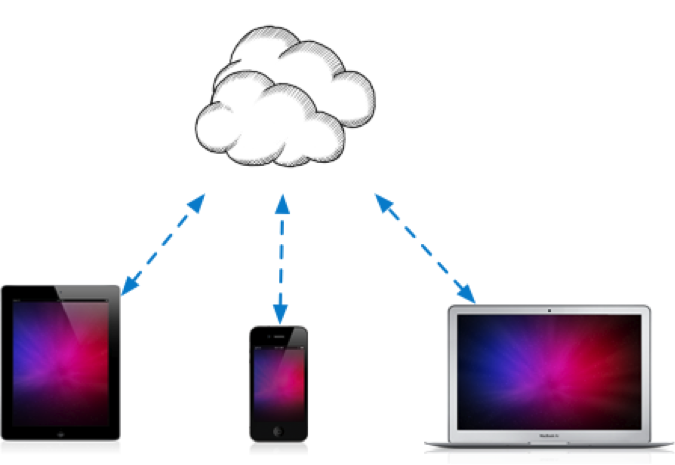
\includegraphics{Motivation_1.png}
\caption{Diagram of clients in cloud architecture \label{fig:1}}
\end{figure}

In the cloud architecture, client is the device that connects to the internet to access software in the cloud. Client application is software that runs on client and communicates with the cloud service. In SaaS, the client application is often delivered in form of web application: User can access it using their browser.

However, a web application is not the only solution. For example, on iPhone platform, web applications are limited, they cannot access some hardware features, such as camera. Native applications support these features, and those can be installed via App Store. So a client application can either be a website, or it can be a native application that requires installation.

If there is a native application, in the SaaS business model it is usually free: The company charges users for using the service, not for installing software. If user downloads the free application, but is not subscribed to the service, they are not able to use it.

Atmosphere tries to improve these client applications and make their development faster. The next sections will discuss the current state of client applications.

\subsection{Desktop applications}

With SaaS becoming a popular model for software business, companies focus less on desktop applications. Instead, they build services that work online and the clients use web interface to access these services.

It is possible to build desktop applications for SaaS products. But developing for desktop (for all platforms) takes more time and effort than developing for web. (Which supports all platforms right away.) Building a desktop application for every platform is not a viable option in many cases.

This is not a case for social networks, for example. Social networks have millions of users and provide an API. Therefore many developers try to improve the user experience by building desktop applications for these services.

It seems that user experience is generally better with desktop application rather than web applications. The first reason is that the whole user interface is operating on the client side: That means only the data is transferred through the network. Some desktop applications even use local storage to cache the local data.

The only problem left to solve is the case when application does not work with local data, but always makes networks requests, blocking the interface, needlessly making user wait.

The desktop library of Atmosphere solves this problem by providing a library that extends local storage framework and adds transparent networking without interface blocking. 

One last type of desktop applications are those with purpose of notifying users of events. Should an event occur in a web application, the only way of immediately notifying user is via email. These emails tend to get very annoying after time, so user start creating filters that hide them from the inbox, which partly defies the purpose.

A better way of notifying users is to provide a desktop application they can launch and quit. Part of Atmosphere is the notification server which together with client libraries allow instant notifications for events that occurred in the application. 

\subsection{Mobile applications}

Mobile applications became a very important part of SaaS. It is the time when many users own smartphones with constant connection to the Internet, and they expect every service to provide a mobile application that would allow them to perform the basic tasks using a simplified user interface. \citep{facebook_stats}

Mobile applications have often high priority when a new SaaS product is shipped. In many cases a special, mobile version of the site could solve the fulfill the purpose, but compared to native mobile apps, these lack a great deal of responsiveness and speed.

Also, a native mobile application provides access to hardware-specific features, such as the the camera, GPS, the accelerometers, multi-touch event handling, and others.

Mobile applications have become very popular. \citep{facebook_stats} Compared to desktop applications, they are developed a lot more frequently. Compared to web applications, native mobile applications are much more responsive and faster.

There is a mobile framework RestKit \citep{restkit} that solves a similar problem as Atmosphere for iOS and Mac applications. Its first feature is to simplify working with REST interfaces, but in addition it provides a way of caching remote objects in local storage, similarly to Atmosphere.

The only flaw of this framework is that it does not support creating objects locally, when there is no internet connection. Atmosphere solves this problem by tracking local changes all the time, no matter if user has internet connection or not, and synchronizing them with the web service when the internet connection is available.

Notifications are supported on mobile platforms in different ways. On iOS there is a central notification system, that is managed by Apple infrastructure. \citep{iphone_ipad_book} The application is not responsible for managing open connection to receive notifications, instead when an event occurs on the server side, it notifies the Apple notification service that then delivers notification to the client. This solution is superior to managing connection by every client connection individually. First, it saves the memory footprint, CPU usage, thus it saves battery life. Secondly, the code responsible for managing the connection is provided and well tested by Apple. Network programming is a very unstable, so it would take a lot of effort to come up with solution as reliable as Apple's. 

Atmosphere will not deal with push notifications in a way of receiving notifications when application is not active. But it will apply the same solution of updating objects as soon as they are changed on a different machine to mobile applications. 

\subsection{Web applications}

There is one significant difference between desktop/mobile apps and those that run in a browser. Native apps ship a package of client code that needs to be installed and run on the client platform. Web applications, in contrast, can run anywhere without any installation.

One of the issues of the current web applications is that most of them is just a set of web pages and forms. Some use AJAX to make requests in the background, but there is still occasional page reload.

That requires most of the logic (including fronted logic - logic responsible for rendering user interfaces) on the server side while only the results of requests are delivered to user. This concept is old \citep{html_history} and is being replaced by JavaScript-heavy client side applications that have their own logic, especially for the user interface. They make requests only when necessary - to transfer only the data, not HTML.

This thesis does not explore all of the possible solutions of achieving this goal because there are many various options. Instead, Atmosphere assumes the developer has or is building a JavaScript application.

Moving logic to the client side is already an improvement. But even with that, the problem mentioned before still exist.

For example, TaskDo (one of Atmosphere-based applications, that were built along with the framework), provides an easy way to access user's tasks in Google Tasks. The simple interface consists of two screens: List of ``task lists'' and list of tasks in the list. Without Atmosphere, clicking on a task list would result in a few seconds wait for the tasks inside to load. With Atmosphere, the data is already cached locally, so opening a task list is instant. TaskDo and other applications are described in section Case Study.

The next problem with web applications is that there are no push notifications, unless the business domain explicitly requires them. (Such as a chat application, or a game.) For most applications, it's necessary to update objects  in real time between users, but it would make the application better.